\documentclass[a4paper,14pt]{extreport}
\usepackage[left=1.5cm,right=1.5cm,
    top=1.5cm,bottom=2cm,bindingoffset=0cm]{geometry}
\usepackage{scrextend}
\usepackage[T1,T2A]{fontenc}
\usepackage[utf8]{inputenc}
\usepackage[english,russian,ukrainian]{babel}
\usepackage{tabularx}
\usepackage{amssymb}
\usepackage{color}
\usepackage{amsmath}
\usepackage{mathrsfs}
\usepackage{listings}
\usepackage{graphicx}
\graphicspath{ {./images/} }
\usepackage{lipsum}
\usepackage{xcolor}
\usepackage{hyperref}
\usepackage{tcolorbox}
\usepackage{tikz}
\usepackage[framemethod=TikZ]{mdframed}
\usepackage{wrapfig,boxedminipage,lipsum}
\mdfdefinestyle{MyFrame}{%
linecolor=blue,outerlinewidth=2pt,roundcorner=20pt,innertopmargin=\baselineskip,innerbottommargin=\baselineskip,innerrightmargin=20pt,innerleftmargin=20pt,backgroundcolor=gray!50!white}
 \usepackage{csvsimple}
 \usepackage{supertabular}
\usepackage{pdflscape}
\usepackage{fancyvrb}
%\usepackage{comment}
\usepackage{array,tabularx}
\usepackage{colortbl}

\usepackage{varwidth}
\tcbuselibrary{skins}
\usepackage{fancybox}


\usepackage{tikz}
\usepackage[framemethod=TikZ]{mdframed}
\usepackage{xcolor}
\usetikzlibrary{calc}
\makeatletter
\newlength{\mylength}
\xdef\CircleFactor{1.1}
\setlength\mylength{\dimexpr\f@size pt}
\newsavebox{\mybox}
\newcommand*\circled[2][draw=blue]{\savebox\mybox{\vbox{\vphantom{WL1/}#1}}\setlength\mylength{\dimexpr\CircleFactor\dimexpr\ht\mybox+\dp\mybox\relax\relax}\tikzset{mystyle/.style={circle,#1,minimum height={\mylength}}}
\tikz[baseline=(char.base)]
\node[mystyle] (char) {#2};}
\makeatother

\definecolor{ggreen}{rgb}{0.4,1,0}
\definecolor{rred}{rgb}{1,0.1,0.1}
\definecolor{amber}{rgb}{1.0, 0.75, 0.0}
\definecolor{babyblue}{rgb}{0.54, 0.81, 0.94}
\definecolor{amethyst}{rgb}{0.6, 0.4, 0.8}

\usepackage{float}
\usepackage{wrapfig}
\usepackage{framed}
%for nice Code{
\lstdefinestyle{customc}{
  belowcaptionskip=1\baselineskip,
  breaklines=true,
  frame=L,
  xleftmargin=\parindent,
  language=C,
  showstringspaces=false,
  basicstyle=\small\ttfamily,
  keywordstyle=\bfseries\color{green!40!black},
  commentstyle=\itshape\color{purple!40!black},
  identifierstyle=\color{blue},
  stringstyle=\color{orange},
}
\lstset{escapechar=@,style=customc}
%}


\begin{document}
\pagecolor{white}

%----------------------------------------1
\newtcbox{\xmybox}[1][red]{on line, arc=7pt,colback=#1!10!white,colframe=#1!50!black, before upper={\rule[-3pt]{0pt}{10pt}},boxrule=1pt, boxsep=0pt,left=6pt,right=6pt,top=2pt,bottom=2pt}



\begin{titlepage}
  \begin{center}
    \large
    Національний технічний університет України \\ "Київський політехнічний інститут імені Ігоря Сікорського"


    Факультет Електроніки

    Кафедра мікроелектроніки
    \vfill

    \textsc{ЗВІТ}\\

    {\Large Про виконання лабораторної роботи №2\\
      з дисципліни: «Твердотільна електроніки-2»\\[1cm]

      «ДОСЛ1ДЖЕННЯ ІНТЕГРАЛЬНИХ МДН-ТРАНЗИСТОРІВ» \\

    }
  \bigskip
\end{center}
\vfill

\newlength{\ML}
\settowidth{\ML}{«\underline{\hspace{0.4cm}}» \underline{\hspace{2cm}}}
\hfill
\begin{minipage}{1\textwidth}
Виконавець:\\
Студент 3-го курсу \hspace{4cm} $\underset{\text{(підпис)}}{\underline{\hspace{0.2\textwidth}}}$  \hspace{1cm}Б.\,П.~Фіцай\\
\vspace{1cm}

Превірив: \hspace{6.1cm} $\underset{\text{(підпис)}}{\underline{\hspace{0.2\textwidth}}}$  \hspace{1cm}Л.\,М.~Королевич\\

\end{minipage}

\vfill

\begin{center}
2021
\end{center}
\end{titlepage}
%##########################################-------------1
\begin{center} МЕТА РОБОТИ\\ \end{center}

Вивчення будови, методів виготовлення, основних характеристик і технічних параметрів інтегральних МДН-транзисторів.

\begin{center} ЗАВДАННЯ\\ \end{center}


1.Виконати вимірювання сімейства характеристик передачі - залежності струму стоку від напруги затвор-виток інтегрального МДН-транзистора: $\mathrm{Ic}($ Езв $),$ при Еc=const. Побудувати характеристики передачі на одному малюнку.\\

2.Виконати вимірювання вихідних характеристик - залежності струму стоку від напруги сток-виток: $-\mathrm{Ic}(\mathrm{EcB}),$ при Ез= const Побудувати сімейство вихідних характеристик.\\

3.Побудувати графік залежності $\sqrt{I_{C}\left(E_{3 B}\right)}$ у пологій області вихідних характеристик та графічно визначити порогову напругу МДН-транзистора.\\

4.Визначити крутизну, динамічний опір стоку, коефіцієнт підсилення напруги для крутої для пологої областей вихідних характеристик транзистора $(\mathrm{S} 1 ; \mathrm{S} 2,$ $ \mathrm{rc} 1 ; \mathrm{rc} 2 ; \mu_{1} ; \mu_{2})$\\

5.3апропонуйте заходи щодо підвищення частоти Г$_{\text{верх}}$, зниження порогової напруги та зменшення паразитних ємностей інтегрального МДН-транзистора.\\

%##########################################-------------2
\begin{figure}[h]
\center{\includegraphics[width=1\linewidth]{s.png}}
\caption{установка  К168КТ2А.}
\label{ris1}
\end{figure}



%##########################################-------------3
\begin{figure}[h]
  \begin{center}Табл. 1: Значення для сімейства характеристик передачі.\end{center}
\center{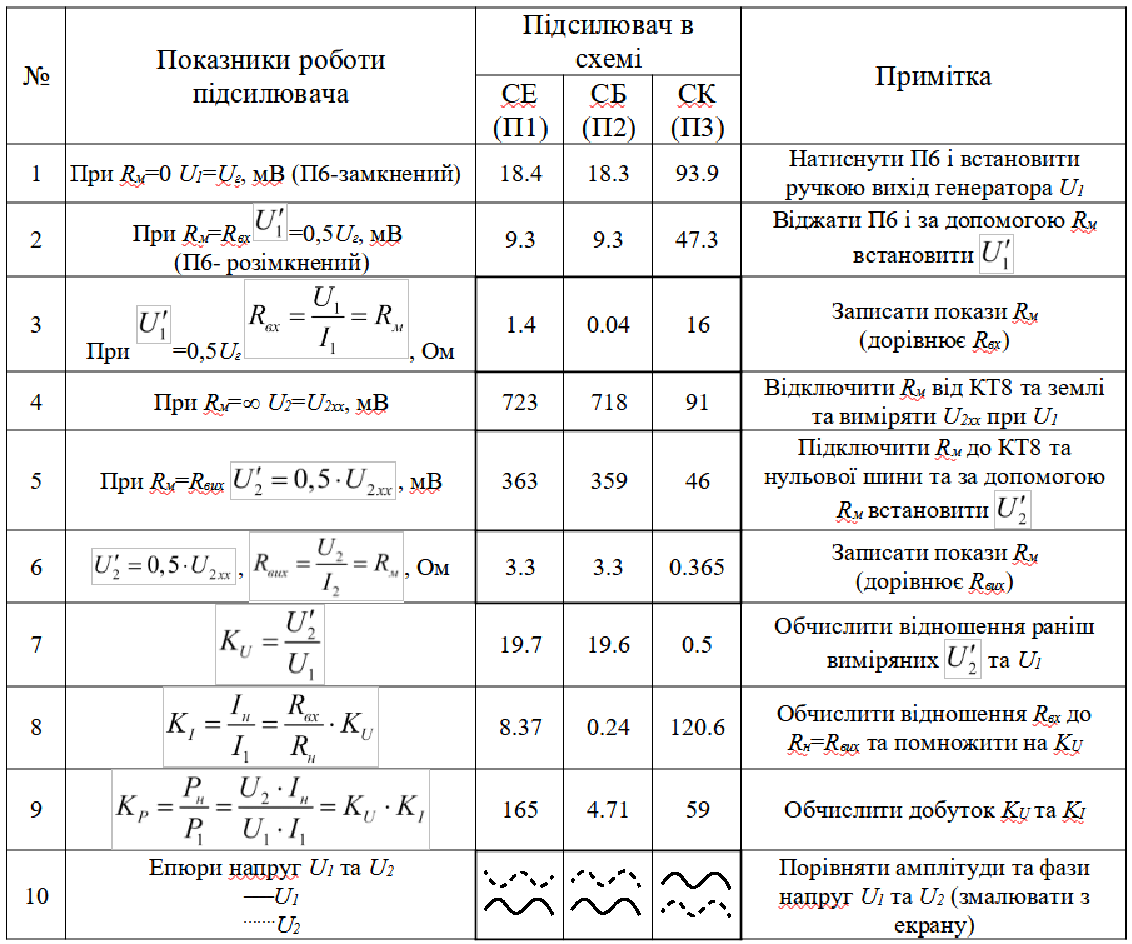
\includegraphics[width=1\linewidth]{t1.png}}

\label{ris1}
\end{figure}
%##########################################-------------4
\begin{figure}[h]
  \begin{center}Табл. 2: Вихідні характеристики, залежності струму стоку від напруги сток-виток.\end{center}
\center{\includegraphics[width=0.8\linewidth]{t22.png}}

\label{ris1}
\end{figure}
%##########################################-------------5


\newpage
\clearpage
\begin{figure}[h]
\center{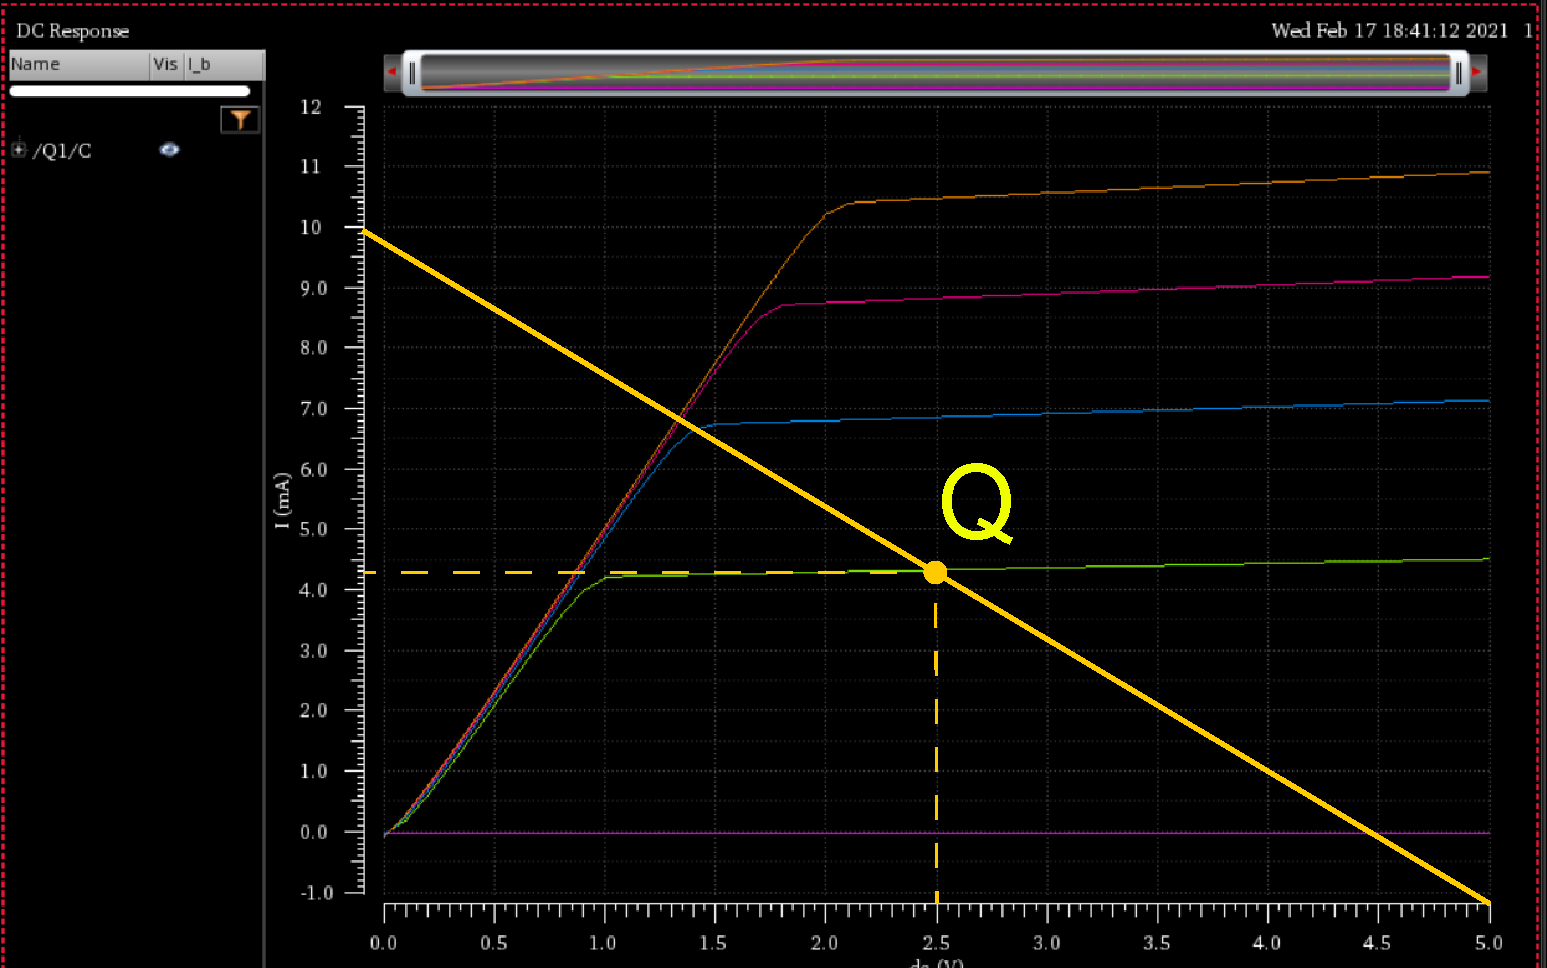
\includegraphics[width=0.8\linewidth]{1.png}}
\caption{Сімейство передавальних характеристик МДН-транзистора}
\label{ris1}
\end{figure}

\begin{figure}[h!]
\center{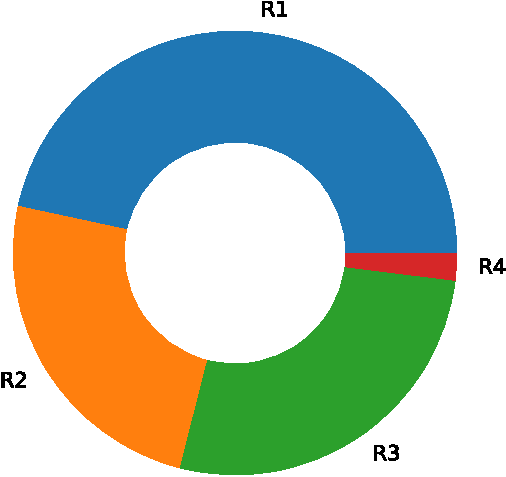
\includegraphics[width=0.8\linewidth]{2.png}}
\caption{Сімейство вихідних характеристик МДН-транзистора}
\label{ris1}
\end{figure}
%##########################################-------------6
\begin{figure}[h]
\center{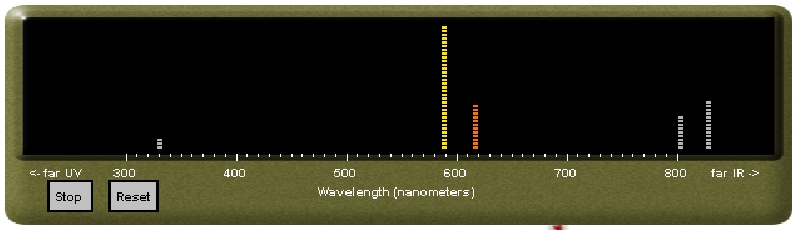
\includegraphics[width=0.7\linewidth]{3.png}}
\caption{Сімейство залежності кореня струму від напруги затвор-витік}
\label{ris1}
\end{figure}
%##########################################-------------7
\newpage
  \begin{center}Розрахунки\end{center}
\begin{align}\label{q1}
  S = \dfrac{\triangle I_C}{\triangle U_{\text{3}}} = \dfrac{6,2-1,4}{5,2-4}=4 \dfrac{\text{мА}}{\text{В}}
\end{align}

\begin{align}\label{q2}
  r_i = \dfrac{\triangle U_{BC}}{\triangle I_{C_2}} =\dfrac{1-0,14}{6,2-3} = 0,268 \text{kОм}
\end{align}

\begin{align}\label{q3}
  \mu_1 = S\cdot r_i = 1,075
\end{align}

\begin{align}\label{q4}
  S = \dfrac{\triangle I_C}{\triangle U_{\text{3}}} = \dfrac{1-0,4}{1,9-0,5}= 0,42 \dfrac{\text{мА}}{\text{В}}
\end{align}

\begin{align}\label{q5}
  r_i = \dfrac{\triangle U_{BC}}{\triangle I_{C_2}} = \dfrac{3-0,4}{0,6-0,3}= 8,6 \text{Ом}
\end{align}

\begin{align}\label{q6}
  \mu_1 = S\cdot r_i = 3,6
\end{align}





%##########################################-------------8
\newpage
\begin{center} ВИСНОВОК \end{center}
У даній лабораторній роботі було виміряно характеристики передачі та вихідні характеристики МДН-транзистора. За отриманими даними ми розрахували такі параметри як: порогова напруга, крутизна, динамічний опір r стоку, коефіцієнт підсилення напруги для лінійної та пологої ділянок ВАХ. Отримані на практиці ВАХ відповідають теоретичним припущенням. На сімействах вихідних характеристик гарно помітна лінійна область зміни, та зона насичення. Сімейства перехідних характеристик зростають, починаючи зі значення порогової напруги. Можна припустити, що для зниження порогової напруги потрібно як підзаслінний шар використовувати нітрид кремнію.



%##########################################-------------9

%##########################################-------------10

%##########################################-------------11













\end{document}
